% OSA KALVOISTA LAINATTU MOOTTORINOHJAUSKURSSILTA, K2010 LUENTO 4

\frame{
\frametitle{Sytytysjärjestelmä}
Ottomoottorissa polttoaine-ilmaseos sytytetään suurjännitekipinällä. Sytytysjärjestelmän tehtävä on sytyttää ilma-polttonesteseos
\begin{itemize}
\item oikealla hetkellä (optimaalinen suorituskyky ja päästöt)
\item luotettavasti (HC-päästöt, käyntihäiriöt).
\end{itemize}
}

\frame {
\frametitle{Sytytysjärjestelmä}
Sytytysjärjestelmän perusperiaate pysynyt samana 1800-luvun lopulta asti: ilman ja polttoaineen seos
sytytetään sähkökipinällä. Moottorinohjauksella vaikutetaan {\bf sytytyshetkeen}.
Sytytyshetken valinta vaikuttaa seuraaviin asioihin
\begin{itemize}
\item moottorista ulos saatava teho
\item polttonesteen kulutus
\item nakuttaako moottori vai ei
\item kuinka puhtaita ovat pakokaasut
\end{itemize}
Kaikkia asioita ei saada parhaaseen mahdolliseen arvoon samanaikaisesti, vaan on tehtävä kompromissi.
Esimerkiksi sytytyksen aikaistaminen lisää moottorin tehoa ja vähentää kulutusta, mutta lisää hiilivety- (HC) ja
typenoksidipäästöjä (NO$\rm _x$).
}

\frame{
\frametitle{Nykyaikainen sytytyksenohjausjärjestelmä}
\begin{itemize}
\item 2000-luvun autoissa sytytyksenohjausyksikkö on integroitu samaan pakettiin polttoaineensuihkutuksen
ohjausyksikön kanssa.
\item ECU = engine control unit.
\item "Kaikki vaikuttaa kaikkeen"
\item Vanhanaikaisiin sytytysjärjestelmiin tutustuminen on kuitenkin havainnollista.
\end{itemize}
}




\frame{
\frametitle{Sytytystulpat}
\begin{itemize}
\item Tulpan elektrodien väliin syttyvä valokaari sytyttää polttoaineilmaseoksen.
\item Tulpan on kestettävä kemiallista rasitusta, korkeita lämpötiloja (jopa 1000 $^\circ$C), korkeita jännitteitä (30 kV)
ja korkeaa painetta (80 bar).
\item Sytytystulppien käyttölämpötilan on oltava suurin piirtein välillä 500 $^\circ$C - 900 $^\circ$C. Liian kylmässä tulppa
ei pala puhtaaksi (oikosulkuvaara), ja liian kuuma lämpötila johtaa voimakkaaseen korroosioon ja hehkusyttymisen vaaraan.
\item Tulpan {\bf lämpöarvo} kertoo, kuinka paljon tulppa lämpenee. Pienen (2...5) lämpöarvoluvun tulppiin johtuu vähän
lämpöä palotilasta. Suuren (7...10) lämpöarvoluvun tulppiin johtuu paljon lämpöä.
\item Väärien tulppien käyttö johtaa esimerkiksi karstoittumiseen (liian kylmät tulpat) tai korroosioon (liian kuumat tulpat).
\end{itemize}
}

\frame{
\frametitle{Sytytysjärjestelmien perusrakenteet}
\begin{itemize}
\item Induktiivinen ja kapasitiivinen akkusytytys.
\item Induktiivinen ja kapasitiivinen magneettosytytys.
\end{itemize}
}

\frame{
\frametitle{Induktiivisten sytytysjärjestemien päätyypit}
\begin{tabular}{ l l p{6cm} }
 & Nimi & Ominaisuudet\\
SZ & Puolasytytys & Sytytysimpulssi, säätö ja kipinänjako mekaanisesti.\\
TZ & Transistorisytytys& Impulssi tuotetaan elektronisesti.\\
EZ & Elektroninen sytytys& Impulssi ja säätö elektronisesti.\\
VZ & Täyselektroninen sytytys& Sytytysimpulssi, säätö ja kipinänjako elektronisesti.\\
\end{tabular}

}

\frame{
\begin{center}
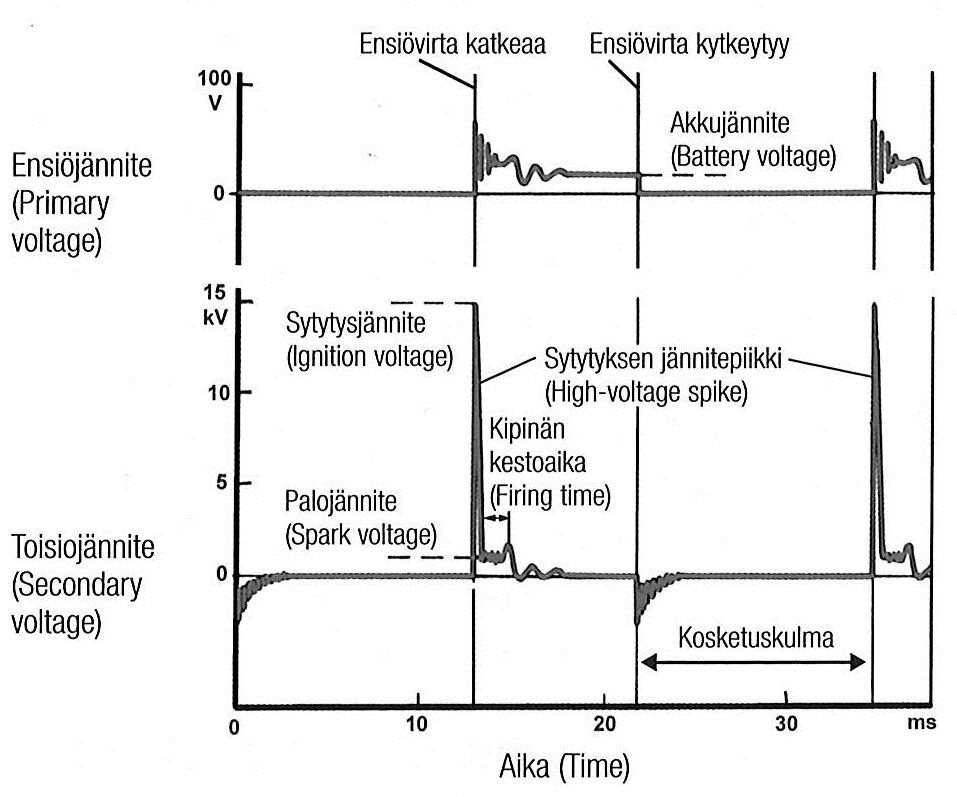
\includegraphics[height=80mm]{sytytysjarjestelma_pics/kayra.png}
\end{center}
\tiny Kuvan lähde: Simo Nieminen: {\em Auton sähkölaitteet}, 1. painos (2008), WSOY, sivu 195.
}

\frame{
\frametitle{Wanhanaikainen puolasytytys (SZ)}
\begin{itemize}
\item Sytytysimpulssi tuotetaan katkaisemalla sytytyspuolan virta katkojan kärjillä.
\item Kun kärjet ovat kiinni, puolan ensiökäämin virta kasvaa (energiaa varastoituu magneettikenttään).
\item Kun virta katkaistaan äkillisesti, toisiokäämiin indusoituu korkeajännite, joka aikaansaa kipinän tulpan kärkien välillä.
\item Suurilla kierrosluvuilla ensiövirta ehtii olla kytkettynä vain vähän aikaa. Magneettikenttään varastoituu vähemmän
energiaa kuin pienillä kierrosluvuilla.
\item Ensiökäämin induktanssin on oltava riittävän pieni, jotta myös suurilla kierrosluvuilla syntyy riittävän suuri jännite.
\item Virtaa rajoitetaan usein etuvastuksella, joka ohitetaan kylmäkäynnistyksessä.
\end{itemize}
}

\frame{
\begin{center}
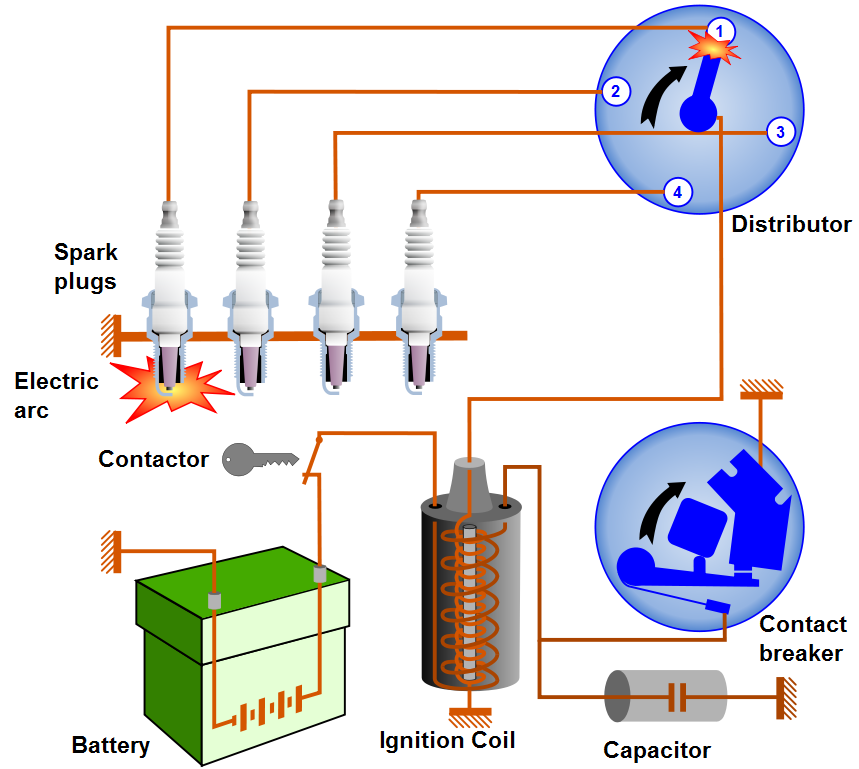
\includegraphics[height=60mm]{sytytysjarjestelma_pics/perus.png}
\end{center}
\tiny Kuvan lähde: \url{http://commons.wikimedia.org/wiki/File:Car_ignition_system.svg}
}


\frame{
\frametitle{Virranjakaja}
\begin{itemize}
\item Virranjakajan tehtävä on jakaa jännitepulssi oikealle tulpalle.
\item Katkojan tehtävä on katkaista ensiövirta oikealla hetkellä (SZ).
\item Nykyaikaisissa sytytys- ja moottorinohjausjärjestelmissä virranjakaja huolehtii ainoastaan
kipinän jakamisesta tulpille.
\item Täyselektronisissa järjestelmissä mekaanista virranjakajaa ei tarvita.
\end{itemize}
}

\frame{
\frametitle{Katkoja}
\begin{itemize}
\item Katkojassa on nokan käyttämä kosketinkärki, joka katkaisee ensiövirran.
\item Kuluva osa, sekä mekaanisesti että kipinöinnin takia (virran katkaiseminen aikaansaa kipinän
myös ensiöpuolella).
\item Sytytyskondensaattori vähentää kipinöintiä ja radiotaajuisia häiriöitä.
\end{itemize}
}

\frame{
\frametitle{Keskipako- ja alipainesäädin}
\begin{itemize}
\item SZ- ja TZ-järjestelmissä virranjakajaan on integroitu säätimet, jotka säätävät sytytysennakkoa
moottorin kuorman ja kierrosluvun mukaan.
\item Keskipakosäädin säätää sytytystä sitä aikaisemmaksi, mitä suurempi on moottorin kierrosluku.
\item Alipainesäädin säätää sytytysennakkoa moottorin kuormituksen mukaan. Pienellä kuormituksella
ennakkoa kasvatetaan, koska seos palaa silloin hitaammin. 
\end{itemize}
}

\frame{
\frametitle{Transistorisytytysjärjestelmä (TZ)}
\begin{itemize}
\item Ero SZ-järjestelmään: ensiövirtaa ei katkota kärkiä läpsyttämällä, vaan elektronisesti.
\item On olemassa myös kärkiohjattuja transistorisytytysjärjestelmiä (TSZ-k), missä kärjet toimivat
anturina mutta varsinainen katkominen tapahtuu transistorin avulla.
\item Käytetyimmät anturityypit ovat induktiivinen impulssianturi (TZ-I) sekä Hall-anturi (TZ-H).
\item Etuja:
\begin{itemize}
\item Ensiövirran rajoitus voidaan tehdä elektronisesti (ei etuvastuksia ym.).
\item Kosketuskulman (kauanko ensiövirta on kytkettynä ennen kipinää) elektroninen säätö.
\item Lepovirran katkaisu (puola ei kuumene, jos moottori on sammutettu mutta sytytysvirta päällä).
\item Ei kuluvia kärkiä.
\end{itemize}

\end{itemize}
}


\frame{
\frametitle{Anturit}
\begin{itemize}
\item Moottorin asentoa mittaavasta sytytysjärjestelmän anturista käytetään myös termiä tahdistin.
\item Anturi voi sijaita virranjakajassa, vauhtipyörän yhteydessä tai kampiakselin etupäässä.
\item Induktiotahdistin: toimii kuten pieni sähkömoottori. Sijoitus virranjakajaan tai vauhtipyörälle.
\item Voidaan käyttää myös Hall-anturiin perustuvaa tahdistinta tai optista tahdistinta.
\end{itemize}
}

\frame{
\begin{center}
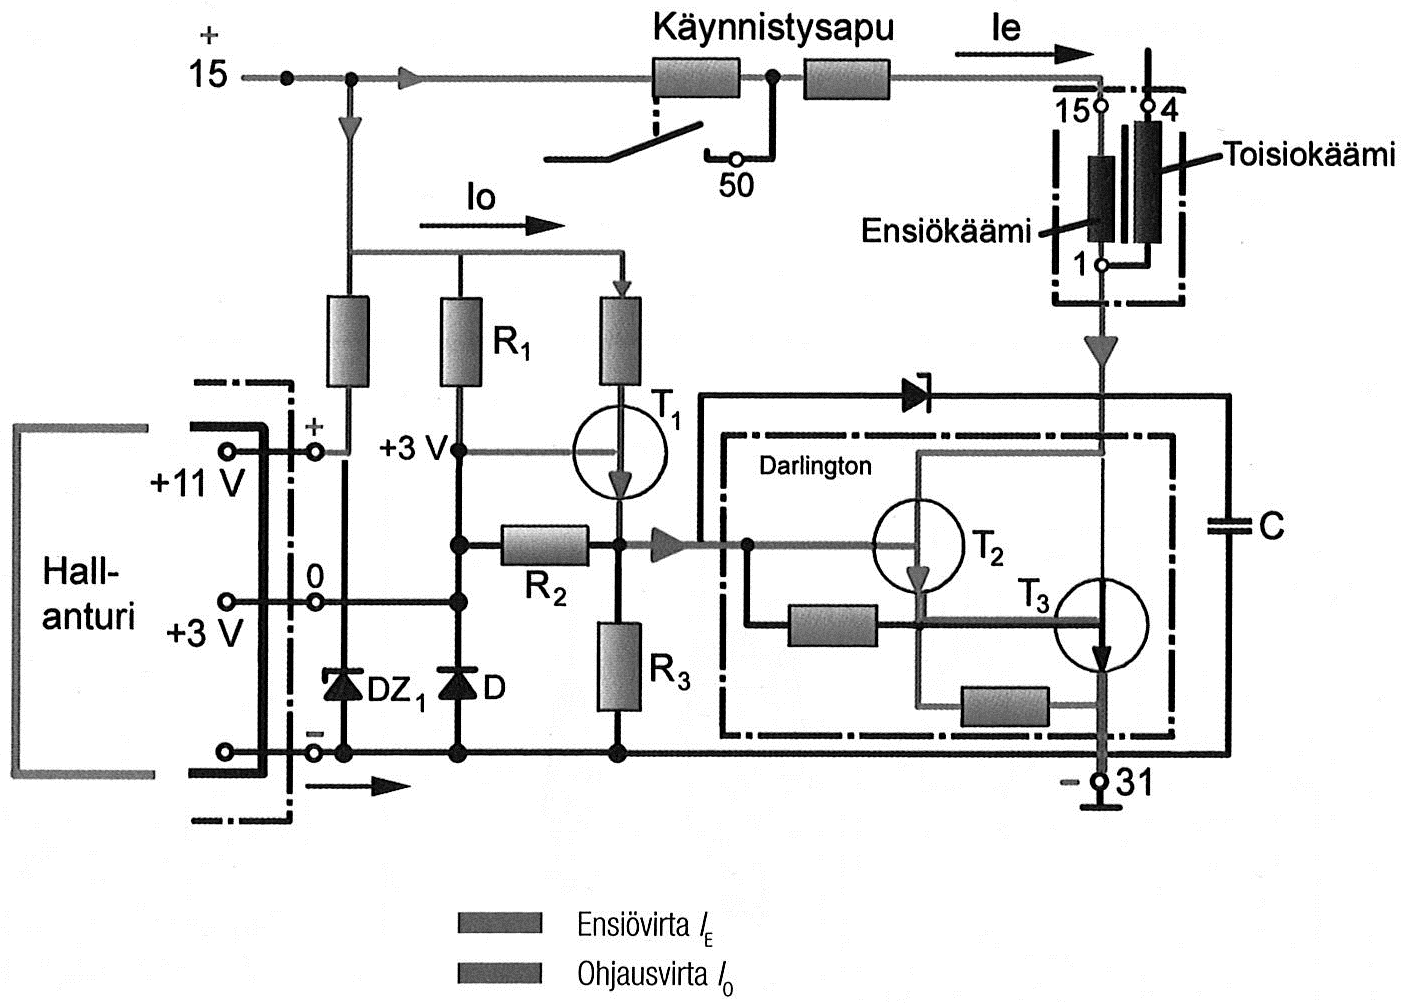
\includegraphics[height=80mm]{sytytysjarjestelma_pics/elektroninen.png}
\end{center}
\tiny Kuvan lähde: Simo Nieminen: {\em Auton sähkölaitteet}, 1. painos (2008), WSOY, sivu 200.
}


\frame{
\frametitle{Elektroninen sytytys (EZ)}
\begin{itemize}
\item Ero TZ-järjestelmään: alipaine- ja keskipakosäädin on korvattu elektronisella säätöyksiköllä.
\item Elektroniikan käyttö mahdollistaa mielivaltaiset säätökäyrästöt.
\item Tietokone laskee oikean sytytyshetken pyörintänopeuden, imusarjan paineen, moottorin ja imuilman lämpötilan ja
akkujännitteen perusteella.
\end{itemize}
}

\frame{
\frametitle{Täyselektroninen sytytys (VZ)}
\begin{itemize}
\item Ero EZ-järjestelmään: virranjakaja korvattu elektronisella kipinänjaolla.
\item Käyttö joko kaksoiskipinäsytytyspuolilla (kipinä sekä puristustahdissa että poistotahdissa olevalle sylinterille) tai
yksittäiskipinäsytytyspuolilla.
\end{itemize}
}

\frame{
\frametitle{Nakutuksen esto}
\begin{itemize}
\item Nakutus = polttoaine syttyy sekä itsestään että kipinästä. Kaksi palamisrintamaa kohtaavat $\to$ paineisku.
\item Nakutus voi tuhota moottorin muutamassa minuutissa.
\item Sytytysennakkoa säädettäessä on jätettävä turvaväli moottorin nakutusrajaan (=ennakko, jolla moottori todennäköisesti nakuttaa).
\item Käyttämällä elektronista nakutuksen tunnistinta, voidaan turvaväliä kaventaa huomattavasti. Nakutukseen voidaan reagoida
välittömästi ($\to$ sytytystä myöhäisemmälle).

\end{itemize}
}



\frame{
\frametitle{Kapasitiivinen sytytys (HKZ)}
\begin{itemize}
\item Kapasitiivisessa sytytysjärjestelmässä sytytysenergiaa ei varata sytytyspuolan käämiin, vaan
kondensaattoriin.
\item Sytytysmuuntajaa tarvitaan edelleen jännitteen nostoa varten.
\item Muuntajan ensiökäämin induktanssi on pieni, jotta energia purkautuu ensiökäämiin nopeasti.
\end{itemize}
}

\frame{
\frametitle{Kapasitiivisen sytytyksen ominaisuuksia}
\begin{itemize}
\item Kondensaattorin varaaminen kestää vain satoja mikrosekunteja $\to$ vahva kipinä myös suurilla käyntinopeuksilla.
\item Lyhyempi kipinän kestoaika; voidaan kompensoida jännitettä ja kärkiväliä kasvattamalla.
\item Tulpan kestoikä pitenee.
\item Suuri jännite lisää läpilyöntiherkkyyttä (kosteus, lika, kuluminen).
\item Monimutkaisempi ja kalliimpi kuin induktiivinen sytytysjärjestelmä.
\end{itemize}
}

\frame{
\frametitle{Toimintaidea}
\begin{itemize}
\item Kondensaattori ladataan 300--500 V jännitteeseen vaihtosuuntaaja--muuntaja--tasasuuntaaja -rakenteen avulla.
\item Kipinän antaminen tapahtuu purkamalla kondensaattori muuntajan ensiökäämin läpi käyttämällä kytkimenä esimerkiksi tyristoria
(tämän takia järjestelmää kutsutaan joskus tyristorisytytysjärjestelmäksi).
\end{itemize}
}

\frame{
\frametitle{Sytytysenergia}
Kondensaattorin kapasitanssi on noin 1 $\uF$. Jos se varataan 300 voltin jännitteeksi, on sytytykseen käytettävissä energiaa
\[
E=\frac{1}{2}CU^2=45\,{\rm mJ}.
\]
}

\frame{
\frametitle{Jakajaton kapasitiivinen sytytys}
\begin{itemize}
\item Jokaisella tulpalla oma pienoissytytysjärjestelmä muuntajineen ja kondensaattoreineen.
\end{itemize}
}

\frame{
\frametitle{Kapasitiivinen magneettosytytys}
\begin{itemize}
\item Perusperiaate sama kuin kapasitiivisessa akkusytytyksessä, mutta kondensaattorin varausenergia otetaan vauhtipyörämagneeton käämistä.
\end{itemize}
}

\frame{
\frametitle{Turvallisuus}
\begin{itemize}
\item Sytytysjärjestelmästä on mahdollista saada sähköisku.
\item Vaaralliset sähkötapaturmat harvinaisia; yksittäinen korkeajännitepulssi ei ole yhtä vaarallinen kuin valtakunnanverkon 50 Hz vaihtojännite.
\item Puolan toisiopuolta ei silti kannata sorkkia, jos sytytysvirta on kytketty (varsinkin vanhoissa järjestelmissä).
\item Uusissa järjestelmissä sytytysmuuntaja on kiinni suoraan tulpan kannassa. Tämä vähentää rf-häiriöitä ja siinä ohessa
lisää turvallisuutta (pitää olla todella sählä, että saa sähköiskun).
\end{itemize}
}
